\chapter{Evaluation} 

% - Weight vs current consumption vs distance
% - Measure start motor overhead and average consumption (show graph?)

\section{Energy Harvesting from RF}

% Remove robot part from this ??
% Do same process with bq25570 evaluation board from ti

%TODO explain that the it's more efficient to remove the wisp energy harvester and only use the one on the robot
\subsection{Experimental Setup}

Small modifications have been made to the WISP to allow the energy harvester on the robot to harvest energy from RF.
The energy harvester, the storage capacitor and the diode to bypass the harvester, were removed from a WISP.
A wire was soldered to the input pin pad of the now removed harvester on the WISP PCB.
This wire was connected directly to the input of the harvester on the robot.

To evaluate the time required for the robot to harvest enough energy a small experiment was done.
Energy was provided to the WISP on the robot trough an Impinj Speedway R1000 RFID reader, which was connected to a Laird antenna.

\subsection{Results}
The robot was placed 20 cm away from the antenna, typically the distance where the most energy is harvested.
On average the robot required 48 seconds fully charge and move away from the reader.

\subsection{Energy Harvesting from Light}
% Casestudy of conditions robot 
% outdoors/indoors/varying light sources/varying solar panels
% Do experiment in sunlight for nuna panel

%The amount of energy that can be harvested from normal office lighting is limited.
Currently the robot harvests energy form light using a small solar panel.
However, there isn't always enough sunlight available to charge the robots in a acceptable time.
To allow the robots to have sub ten second charge times, a lighting setup needs to be created that provides a reasonable amount of uniform light to the area where the robots move around.
In this section the charge time of the supercapacitor is evaluated, while it's charged from different solar panels and different light sources.

\subsection{Experimental setup}
% Temperature and Light intensity?
To accurately measure the power that is harvested from each solar panel all the experiments were preformed in a darkroom.
The setup consists of a light source that can be positioned at multiple distances from a solar panel.
The solar panel is connected to input of the harvester on the PCB of the robot and when the voltage in the supercapacitor reaches the threshold the buck converter of the energy harvester is enabled.
Voltage is supplied to the WISP which is programed to only enable a GPIO port and enable a LED.
A Saleae Logic, logic analyzer is connected to the port and used to record the time required to charge the capacitor from the minimum to the maximum value.
The port is enabled the light source is disabled and the LED is used to drain the energy from the capacitor.
When the led turns off, indicating that a new charge period begins, the light source is enabled again.
Now a more detailed description will be given of the different components that were tested.

\subsubsection{Solar panels}
Three different solar panels were tested in this experiment, each different in composition, efficiency and panel size, as can be seen from Table \ref{tab:solar_panels}.

%TODO Why these lamps?
\subsubsection{Lamps}
Low cost solar simulators can consist of a combination of LED and halogen light bulbs to simulate sunlight and are used to test the performance of solar panels~\cite{grandi_tia_2014}.
However, in this case the goal is to have a controlled uniform lighting environment where the robots have roughly constant charge times.
Solar panels do not only harvest energy from the visual light spectrum but harvest almost at least as much from the infrared light spectrum, therefore not only light but also heat will shorten the charge time.
Halogen lamps have a lower color temperature than the sun but also emit waves far into the infrared spectrum.
The light sources used in this experiment are a 60W halogen bulb, a 120W halogen halogen bulb and two 150w IR heat lamps where one is colored red.

\subsubsection{Measurements}
Three charge time measurements were preformed, each lamp was positioned 10cm, 30cm and 50cm from the solar panels.
Additionally, for these three distance the temperature was measured at the solar panel using a K-type thermocouple supplied with an Extech EX330 multimeter and the light intensity using the luxmeter on a MASTECH MS8229 multimeter.

\begin{table}[t]
	\centering
	\begin{threeparttable}
		\caption{The solar panels tested in the experiment}
		\label{tab:solar_panels}
		\small
		\begin{tabular}{|l|l|l|l|}
			\hline
			& Composition & Efficiency & Dimensions \\
			\hline \hline
			Banggood \cite{bangood_solar_2017}& Poly-Si & 17\% & 40x30mm \\
			INYS SLMD121H04L-ND\textsuperscript{1}& Mono-Si & 22\% & 43x34mm \\
			Azurspace 3G28C & Triple Junction GaAs& 28\% & 80x40mm \\
			\hline
		\end{tabular}
	\begin{tablenotes}
		\small
		\item [1] Two panels in parallel
	\end{tablenotes}
	\end{threeparttable}
\end{table}

\subsection{Results}
% No difference between the heatlamps in power consumed
% Halogen distributes the light more even
% Panel from nuna
% Refer to appendix for temperature and light data?

Both the temperature and illumination increase by decreasing the distance between the light source and the solar panel. 
Secondly, increasing the output power of the lamp increases temperature and illumination as well. 
However the charge times 
A thing to note is that the both the 60w and 150w ir lamps have a spherical design. This creates a uneven circular shadowing pattern on the surface the lamps are shining on, which becomes more significant on the bigger distances in this experiment.
The 120w lamp has a tubular design and in combination with the light fixture most of the light is reflected down with minimal shadowing of the lamp resulting in a more even light distribution.

\begin{figure}
	\centering
	\begin{subfigure}[b]{0.49\textwidth}
		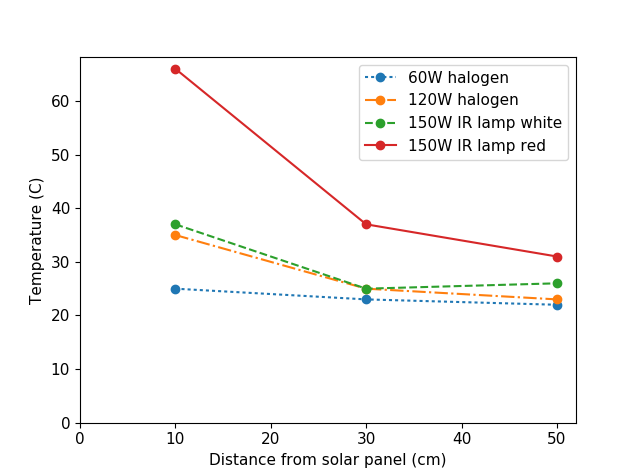
\includegraphics[width=\textwidth]{pics/light_experiment_temp.png}
		\caption{Temperature at different distances}
		\label{fig:light_temp}
	\end{subfigure}
	\begin{subfigure}[b]{0.49\textwidth}
		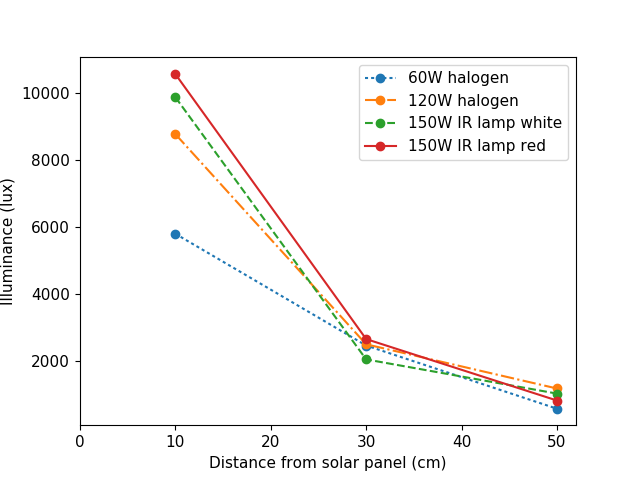
\includegraphics[width=\textwidth]{pics/light_experiment_lux.png}
		\caption{Light intensity at different distances}
		\label{fig:light_lux}
	\end{subfigure}
	\caption{}
\end{figure}


\begin{figure}
	\centering
	\begin{subfigure}[b]{0.49\textwidth}
		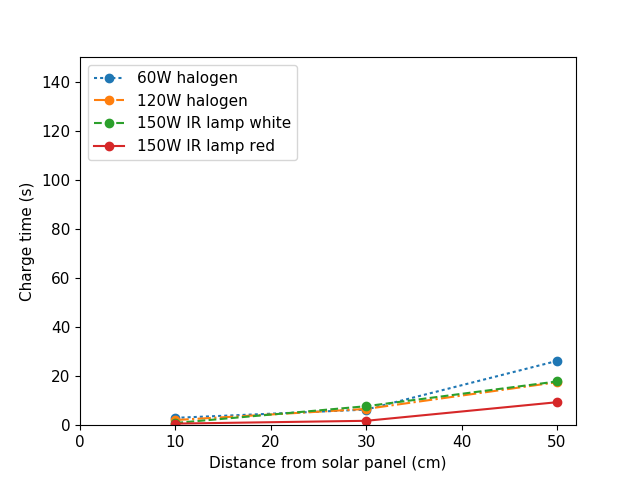
\includegraphics[width=\textwidth]{pics/light_experiment_figure1.png}
		\caption{Ebay panel}
		\label{fig:light_exp1}
	\end{subfigure}
	\begin{subfigure}[b]{0.49\textwidth}
		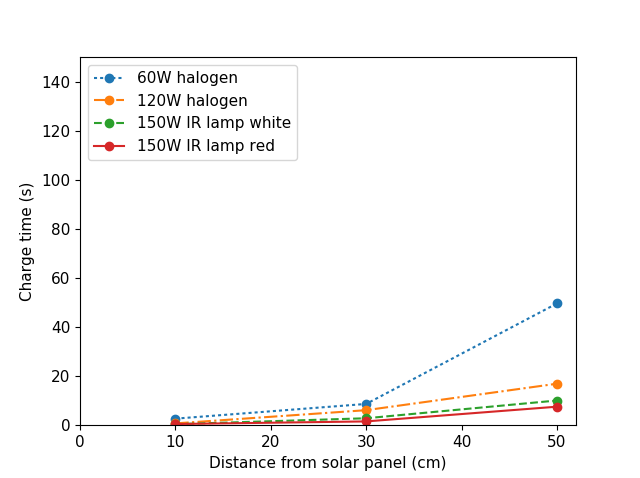
\includegraphics[width=\textwidth]{pics/light_experiment_figure2.png}
		\caption{IXYS SLMD121H04L-ND}
		\label{fig:light_exp2}
	\end{subfigure}
	\begin{subfigure}[b]{0.49\textwidth}
		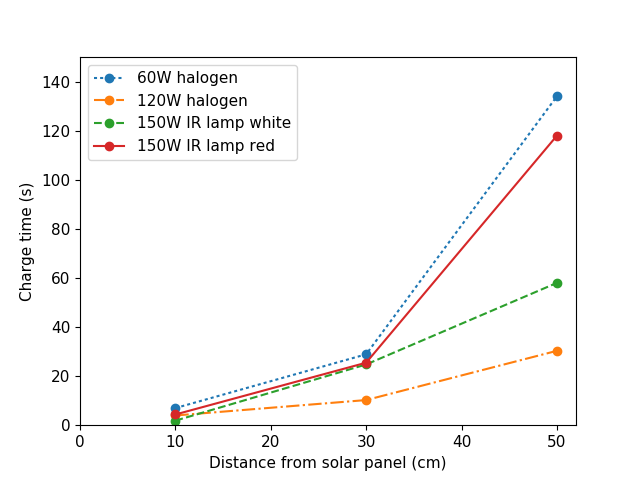
\includegraphics[width=\textwidth]{pics/light_experiment_figure3.png}
		\caption{Azurspace 3G28C}
		\label{fig:light_exp3}
	\end{subfigure}
	\caption{The performance of three different solar panels for different distances from different light sources. The data charge times for the last two are normalized with respect to the surface covered by the first panel.}
\end{figure}

\newpage

\section{Controlled Movements}
\label{sec:controlled_movements}

% Comparison deadreckoning accuracy of battery powered robot with solar powered robot

% Try at least one more supercapacitor: 10mF
% Study reducing the frequency of power interrupts ie smaller energy buffer.
% How does this effect the accuracy of locomotion?
% Can the frequency of power interrupts be related to the 

% Video of robot movement

Now that a variety of solar panel / light combinations has been evaluated, the next Section will evaluate the accuracy of movement of the robot and will compare the battery-less robot and it' battery powered equal.

\subsection{Experimental setup}

To be able to compare the accuracy of the robot while it is exposed to increasingly smaller power cycles, a variety of movements is recorded using a overhead camera.
A camera stand with DSLR camera is positioned on a tabletop and in the camera's view the corners of a square of 80 x 80 cm are indicated with a black marker, see Figure \ref{fig:movement_setup}.
This square can later be used as a reference to convert the robots movement from pixels to cm.
Three different movements are compared, while the robot is moving straight movement of 75 cm, a circle with radius of 30cm and a square of 50 by 50 cm.

\subsubsection{Artificial Power Interrupts}

%TODO Why bat powered
During the experiment the robot will be powered from a battery and power interrupts, i.e the capacitor running out of energy are created artificially using a timer that resets the MCU.
The MSP430FR5969 has the functionality to enable a brownout reset trough software which is used to simulate the event of the supply voltage dropping below the required operating voltage.
With a capacitor of 22mF the robot can operate around 1 second, this resulted in the chosen interrupt periods.
Choosing a period smaller than half a second resulted in uncontrolled behavior, while the control loop was not able to stabilize the movement before the robot runs out of energy again.
Therefore the power interrupt periods evaluated in this experiment are: 1.25 s, 1 s, 0.75 s and 0.5 s.

\subsubsection{Velocity calibration}

%TODO make table with standard deviation of distance traveled 
Each movement is executed at three different PWM target settings: 40\%, 65\% and 90\% of the maximum duty cycle.
To let the robot move a particular distance, the average speed needs to be estimated for each PWM target and power interrupt period.
This is achieved by first determining the time that the robot requires to move approximately 150 cm for each target without power interrupts.
When the robot experiences power interrupts the average velocity of a active period becomes lower due to frequent acceleration from standstill.
With power interrupts the runtime is increased to make the robot travel roughly the same distance.
Finally, the average of five measurements is computed and divided by the commanded runtime of the robot to acquire an average speed for each combination.


\subsubsection{Tracking the Movement}

The robot is programmed to preform the movement at a desired PWM target and optional power interrupt period.
Before the robot executes the movement a green led is enabled on top of the robot, this bright green dot will be the reference point that the tracking software will try to follow.
The camera is used to record the movement which is analyzed using Python and OpenCV 3.2, an example of a tracked movement can be seen in Figure \ref{fig:movement_example}.

\begin{figure}
	\centering
	\begin{subfigure}[b]{0.45\textwidth}
		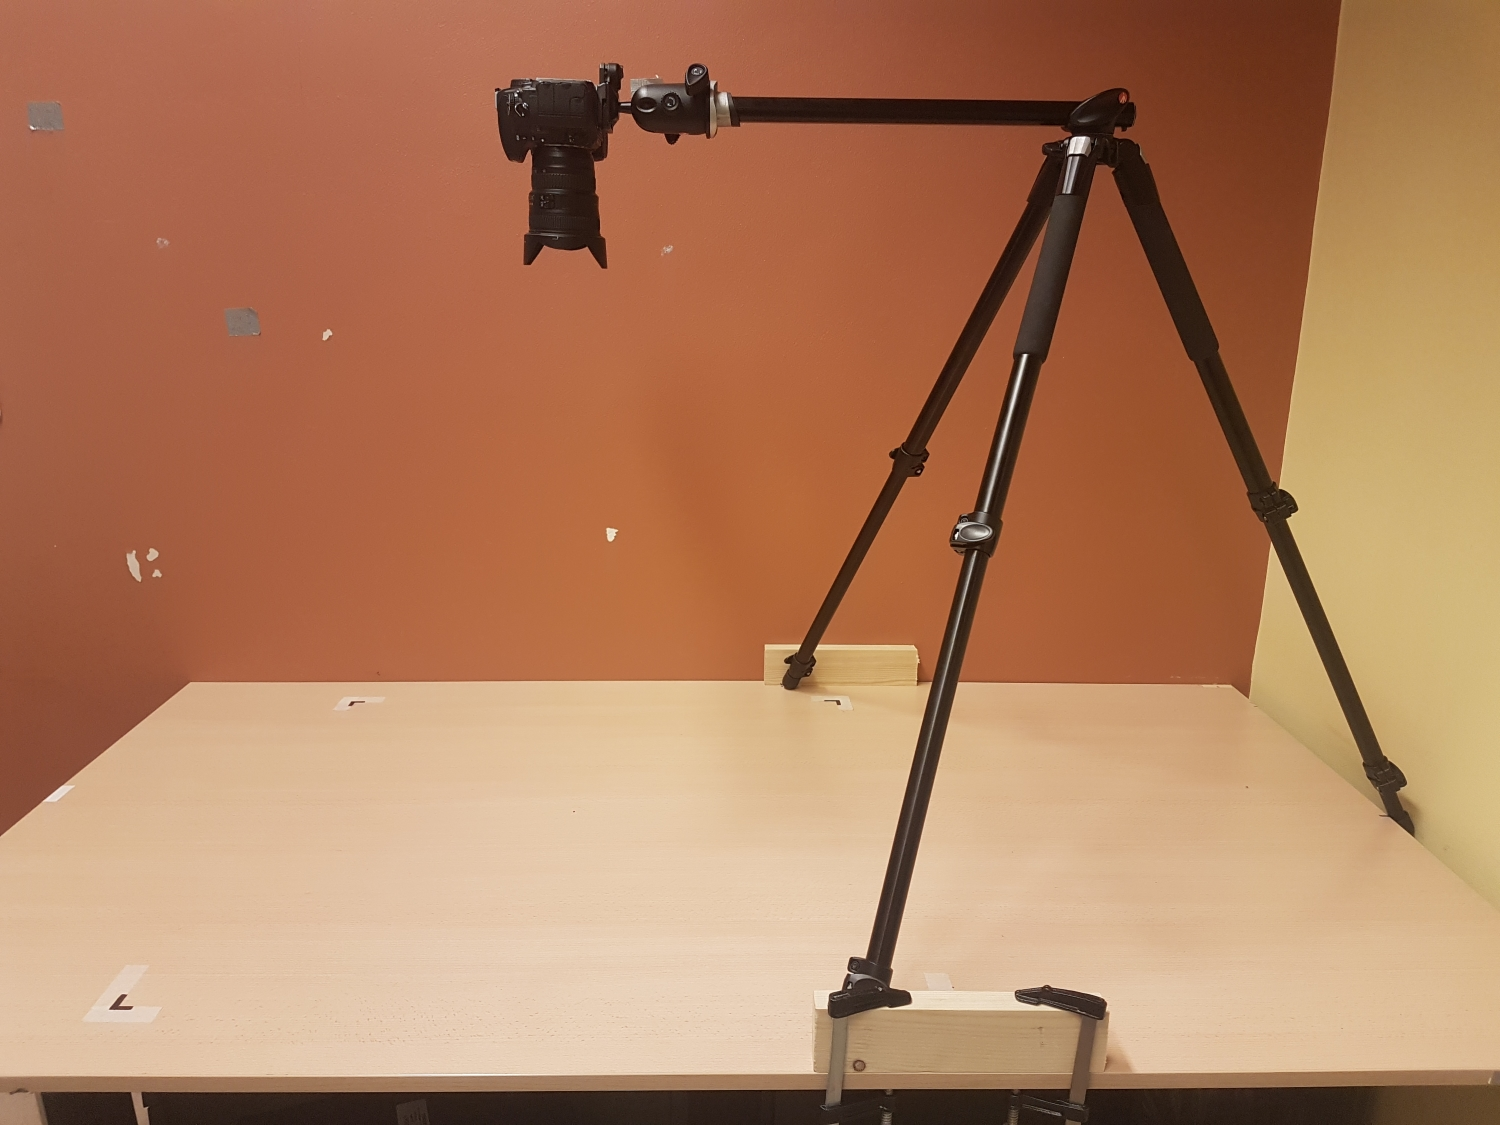
\includegraphics[width=\textwidth]{pics/movement_setup.jpg}
		\caption{Camera setup}
		\label{fig:movement_setup}
	\end{subfigure}
	\quad
	\begin{subfigure}[b]{0.45\textwidth}
		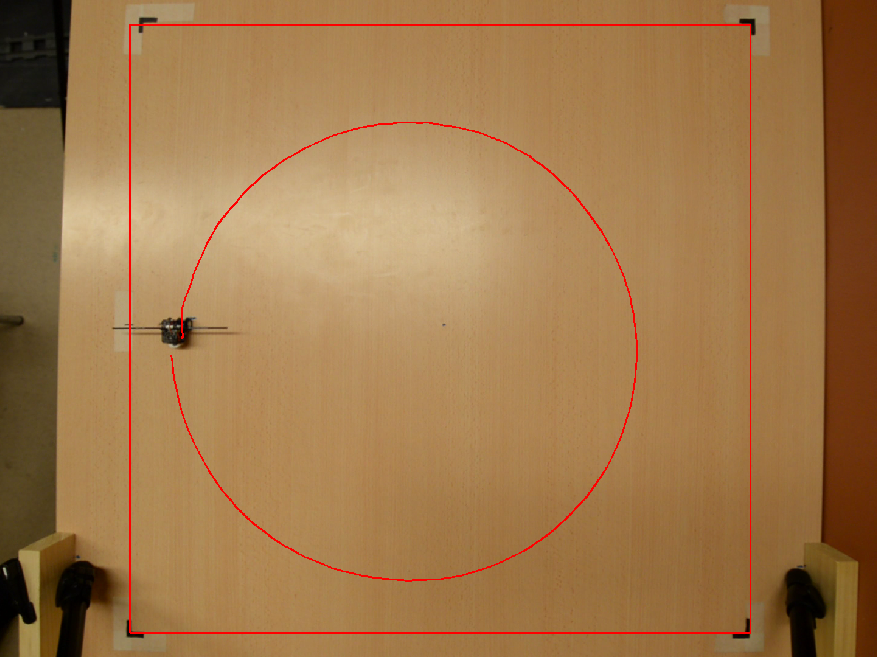
\includegraphics[width=\textwidth]{pics/movement_example.png}
		\caption{Tracking with OpenCV}
		\label{fig:movement_example}
	\end{subfigure}
	\caption{Recording the robots movement}
\end{figure}


\subsection{Movement Accuracy Metrics}

\begin{itemize}
	\item average curvature of straight line movement
	\item Circle plot, make reference flat and plot difference between measured circle and reference (deviation from ideal circle for circular movements)
	\item for both straight and curved movements: length of the total movement and  standard deviation in length of movement
\end{itemize}


\subsection{Straight Movements}

The robot is commanded to move 75cm

\begin{figure}
	\centering
	\begin{subfigure}[b]{0.62\textwidth}
		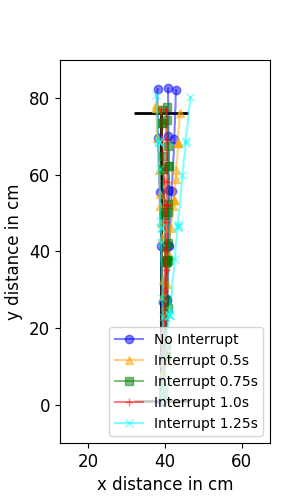
\includegraphics[width=\textwidth]{pics/straight_40.png}
		\caption{Target 40\%}
		\label{fig:stra_exp1}
	\end{subfigure}
	\begin{subfigure}[b]{0.62\textwidth}
		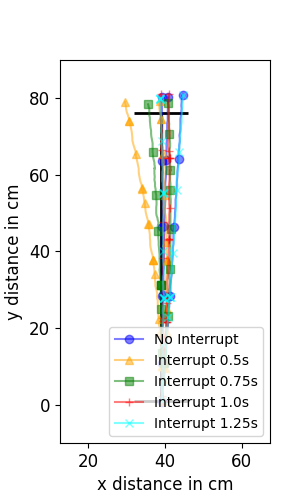
\includegraphics[width=\textwidth]{pics/straight_65.png}
		\caption{Target 65\%}
		\label{fig:stra_exp2}
	\end{subfigure}
	\begin{subfigure}[b]{0.62\textwidth}
		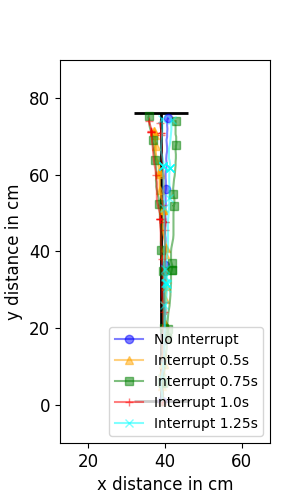
\includegraphics[width=\textwidth]{pics/straight_90.png}
		\caption{Target 90\%}
		\label{fig:stra_exp3}
	\end{subfigure}
	\caption{Straight movements, black horizontal lines show the begin and endpoints}
\end{figure}


\subsection{Circular Movements Results}

The robot is commanded make a circle with radius of 30cm


\begin{figure}
	\centering
	\begin{subfigure}[b]{0.62\textwidth}
		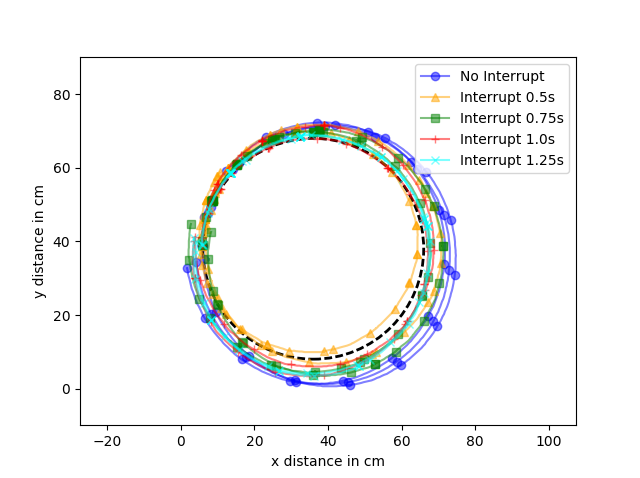
\includegraphics[width=\textwidth]{pics/circle_40.png}
		\caption{Target 40\%}
		\label{fig:circ_exp1}
	\end{subfigure}
	\begin{subfigure}[b]{0.62\textwidth}
		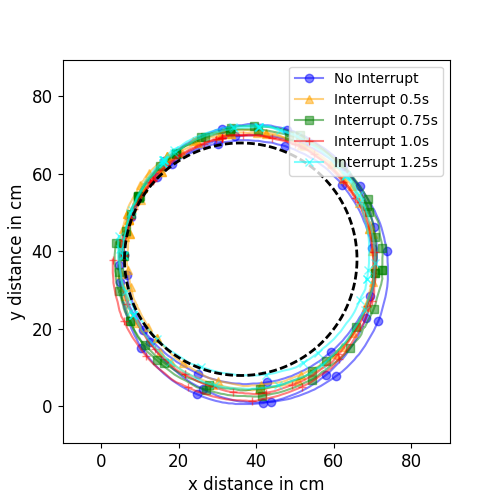
\includegraphics[width=\textwidth]{pics/circle_65.png}
		\caption{Target 65\%}
		\label{fig:circ_exp2}
	\end{subfigure}
	\begin{subfigure}[b]{0.62\textwidth}
		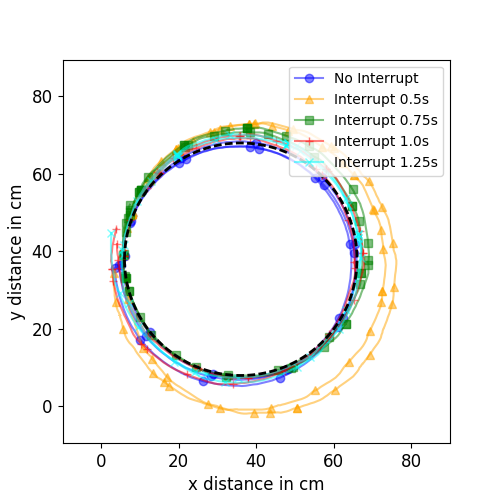
\includegraphics[width=\textwidth]{pics/circle_90.png}
		\caption{Target 90\%}
		\label{fig:circ_exp3}
	\end{subfigure}
	\caption{Circular movements, black dashed circle is the target}
\end{figure}


%\subsection{Results}
%Higher speed + more interrupts results in more drift to the left, because of wheel more in the back or weaker motor?
%How the interrupts are distributed over the distance has a influence or how the last interrupt ends up..
%Lower speed and less interrupts results in a higher accuracy??


%For square: Turn\_right speed should be high enough to turn within 0.5 sec

